
\begin{exr}{}
\begin{center}
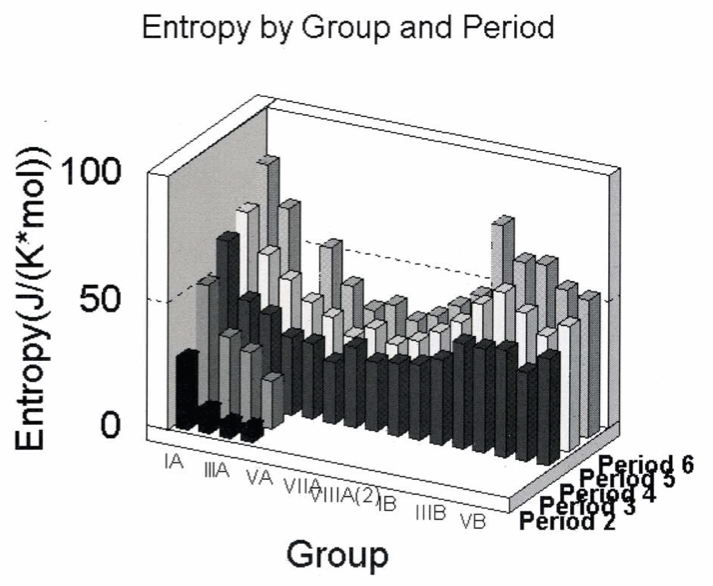
\includegraphics[scale=0.8]{EntropyPT.png}
\end{center}

La Figura mostra l'entropia normal $S^{\circ}_{298}$ per a elements de la taula periòdica, exclosos elements poliatòmics i que no formen sòlids.\cite{thoms_periodic_1995} Pots explicar:
\begin{enumerate}
\item perquè l'entropia augmenta en augmentar el període ($n$ més gran);
\item perquè l'entropia decreix al centre de cada període;i
\item quin és l'efecte d'un augmemnt de l'empaquetament o del grau de coordinació dels elements en l'entropia?
\end{enumerate}
\end{exr}
